\section[Magnetic Order]{\hyperlink{toc}{Magnetic Order}}

\begin{itemize}
    \item spontaneous or under the infl of some \textbf{interactions}: all the spins line up in the same direction even without an external magnetic field
    \item ex. ferromagnet, antiferromagnet, and ferrimagnet.
    \item best ex of ferromagnet is Iron
    \item above a particular temp, spins tend to align randomly and there is a transition at the so called Curie Temperature to a paramagnetic behaviour.
    \item spin in the same direction reduces the energy and so is favourable for the system
    \item Spin-Spin interactions of localised spins we have the \textbf{Heisenberg Hamiltonian}
    \[ -J \sum_{\braket{i,j}}  \textbf{S}_i \cdot \textbf{S}_j , \qquad J>0\]
    and $\textbf{S}_i$ is the spin operator for the ith spin and $\braket{i,j}$ denotes the sum over all neighbouring spins.
    \item Also \textbf{Antiferromagnet} ordered at low Temp, but with zero magnetisation.
    \item discovered by Louis Neel in the 1930s (thus we get Neel Order).
    \item \textbf{Heisenberg Hamiltonian} is very similar but without the negative sign:
    \[ J \sum_{\braket{i,j}}  \textbf{S}_i \cdot \textbf{S}_j , \qquad J>0\]
    \item i.e. alternating spins (up-down-up-down-...) results in minimizing the energy.
    \item if the lattice is triangular you get a \textbf{frustrated magnet} because there are lattice sites that you cannot optimize the lowest energy very well. i.e. think of triangular lattice.
    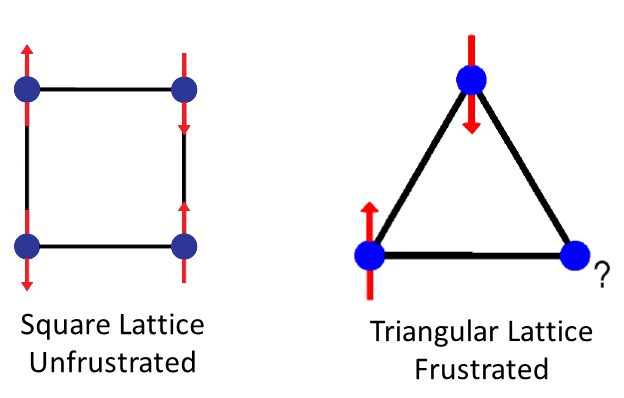
\includegraphics[width= 0.5\linewidth]{Images/Frustration.png}
    \item \textbf{Ferrimagnetism}: 'weak form of ferromagnetism', spins allign within one sublattive but oppose each other on other sublattices. Normally a net magnetic field but typically weaker.
    
    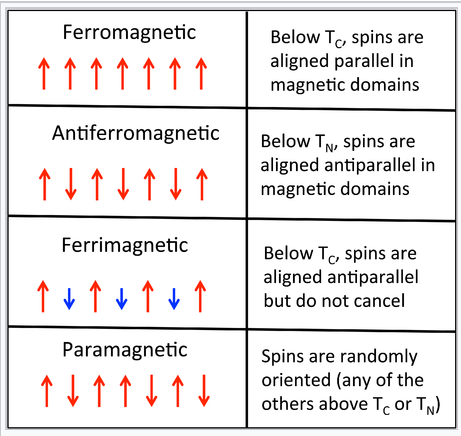
\includegraphics[width = 0.5 \linewidth]{Images/magnetic order.png}
    
    \item Also possible order called canted antiferromagnet and helical spin array.
    
    \item How to detect magnetic order?
    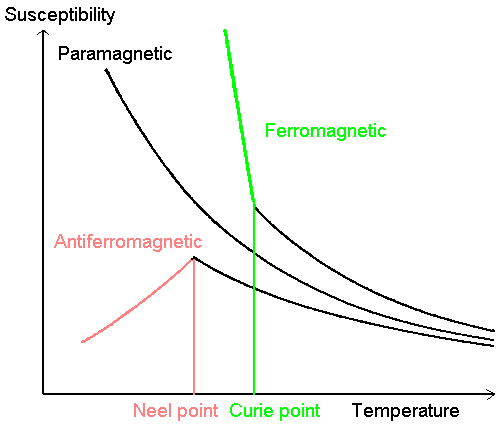
\includegraphics[width  = 0.5 \linewidth]{Images/magnetic chemistry.png}
    \item Measure how magnetic susceptibility changes as you decrease the temperature. Find possible critical temperatures to see deviant behaviour. At high temps they all behave like a paramagnet.
    \item Neutron Scattering Experiment (neutrons have spin): the moments of the neutrons will overlap with the atoms. Interactions with the spin up atoms will be different than the spin down atoms. So you can measure the lattice spacing between spin up or down atoms and see how it increases or decreases with decreasing temperatures. This can show you if it became antiferromagnetic (bigger lattice constant, that is between the atoms of the same spin) or ferromagnetic (smaller lattice constant).
    
    \item \textbf{Domains and Hysteresis:}
    \item \textbf{Annealing}: to make a ferromagnet, hold it at a high temperature and slowly lower the temperature while applying a strong magnetic field in one direction.
    \item \textbf{Magnetic domains} separated by \textbf{domain walls}: If it is cooled down too quickly or the field is too weak, then symmetry can be broken differently in different regions.
    \item \textbf{Quench}: Changing a parameter such as temperature quickly across a transition.
    
    \item Domain walls normally occur over a small region and involve the spin gradually rotating from the value of one domain to that of another (energy is minimized). We then have the bloch (rotation through the plane) and neel (rotation in the plane) walls:
    
    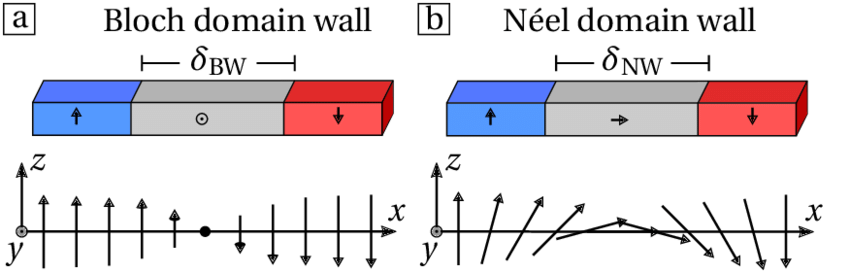
\includegraphics[width = 0.9\linewidth]{Images/domain walls.png}
    
    \item For instant change we get an energy cost of: $\Delta U = JS^2 $
    
    \item For a domain wall of finite width we get: $\Delta U = JS^2 (1- \cos\theta), \quad \theta = \frac{\pi}{N}$ since the spins change by 180 degrees in N spin steps. If we only consider this it would seem the wall would extend to infinite. Therefore we find an extra anisotropy term:
    
    \[ \Delta U = +JS^2 \frac{N}{2} \left( \frac{\pi}{N} \right)^2 + KN \]
    
    Where K = anisotropy term
    \item Average width of the wall is around 150 lattice constants for iron and other ferromagnets.
    
    \item Size of domains walls can be seen as a trade off between energy cost of spins not being aligned (worse if the interactions are stronger), and the preference of the crystal to have particular spin directions (not diagonal: the anisotropy energy).
    
    \item \textbf{Domain wall pinning}: tendency of domain walls to intersect where the defects are in the crystal to minimize the overall energy.
    
    \item \textbf{"Hard Ferromagnet" = Nonzero Hysteresis Loop}.
    
    We observe hysteresis in magnetic susceptibility -- there is typically residual magnetisation when the field is changed.
    
    \item \textbf{Magnetic Force Microscopy (MFM):} Resolution ~ 10-100 nm
    
    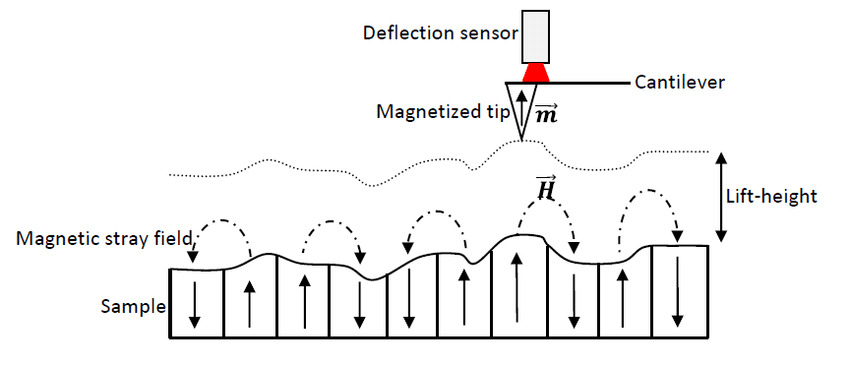
\includegraphics[width = 0.9\linewidth]{Images/MFM.jpeg}
    
    \item Also Atomic Force Microscope (AFM) used for non magnetic samples. Can identify individual atom lattice sites if tuned well. External vibration frequency from the cantilever removes noise (mechanical lock-in technique).
    
    \item Many Types of Resonance Phenomena/ Instruments
    
    \item \textbf{Information Gained:}
    \begin{itemize}
        \item Fine structino of absorption: Electronic structure of individual defects.
        \item Change in line width: Motion of the spin or its surroundings
        \item Chemical or Knight shift: Internal Magnetic field felt by the spin.
        \item Collective spin excitations.
    \end{itemize}
    
    \textbf{Main Applications with Nuclear Magnetic Resonance:} 
    \begin{itemize}
        \item Identification and structure determination for organic / biochemical co
        \item Medical (MRI)
    \end{itemize}
    
    \item \textbf{NMR}:
    
    Nucleus with a magnetic moment \textbf{$\mu$} and angular momentum \textbf{I}.
    
    \[\mu = \gamma \hbar I, \qquad \gamma = \textbf{gyromagnetic ratio} \]
    
    Resonance at:
    
    \[\omega_0 = \gamma B_0 \]
    
    \item Signal Detection (via RF coil)
\end{itemize}
